% ==========================================
% BAB IV PERANCANGAN
% ==========================================
\cleardoublepage
\chapter{PERANCANGAN}
\vspace{-2cm}
\label{chap:desain-konsep-solusi}

\section{Model Konseptual Solusi yang Diusulkan}
Berdasarkan analisis masalah dan pemilihan solusi pada bab sebelumnya, penelitian ini mengusulkan arsitektur sistem hibrida yang mengintegrasikan \textit{Machine Learning} (ML), \textit{Explainable Artificial Intelligence} (XAI), dan \textit{Large Language Model} (LLM) berbasis \textit{Retrieval-Augmented Generation} (RAG).
Sistem ini dirancang dengan arsitektur yang memfasilitasi pengunaan baiik oleh pasien secara mandiri maupun oleh tenaga medis. Aplikasi ini menerapkan mekanisme pengumpulan data yang adaptif bergantung pada konteks pengunaan. Dalam skrining mandiri di rumah, pasien dapat melakukan deteksi dini risiko hipertensi dari rumah tanpa perlu mengunjungi fasilitas kesehatan fisik. Pada mode ini, sistem membatasi kuesioner hanya pada variabel non-invasif saja seperti demografi, gaya hidup, dan riwayat gejala, serta meniadakan parameter klinis yang membutuhkan alat medis atau tindakan invasif seperti pengukuran tekanan darah atau pengambilan sampel darah. Sebaliknya, aplikasi juga dapat digunakan dengan alat ukur tensi di rumah, atau di fasilitas kesehatan, karena terdapat opsi untuk menyertakan veriabel data klinis dan invasif.
Gambar \ref{fig:konsep-solusi} mengilustrasikan desain konsep solusi yang dirancang untuk mengubah data klinis pasien menjadi prediksi risiko yang akurat, transparan, dan mudah dipahami.

\begin{figure}[H]
    \centering
    % Pastikan nama file tidak menggunakan spasi. Gunakan underscore atau dash.
    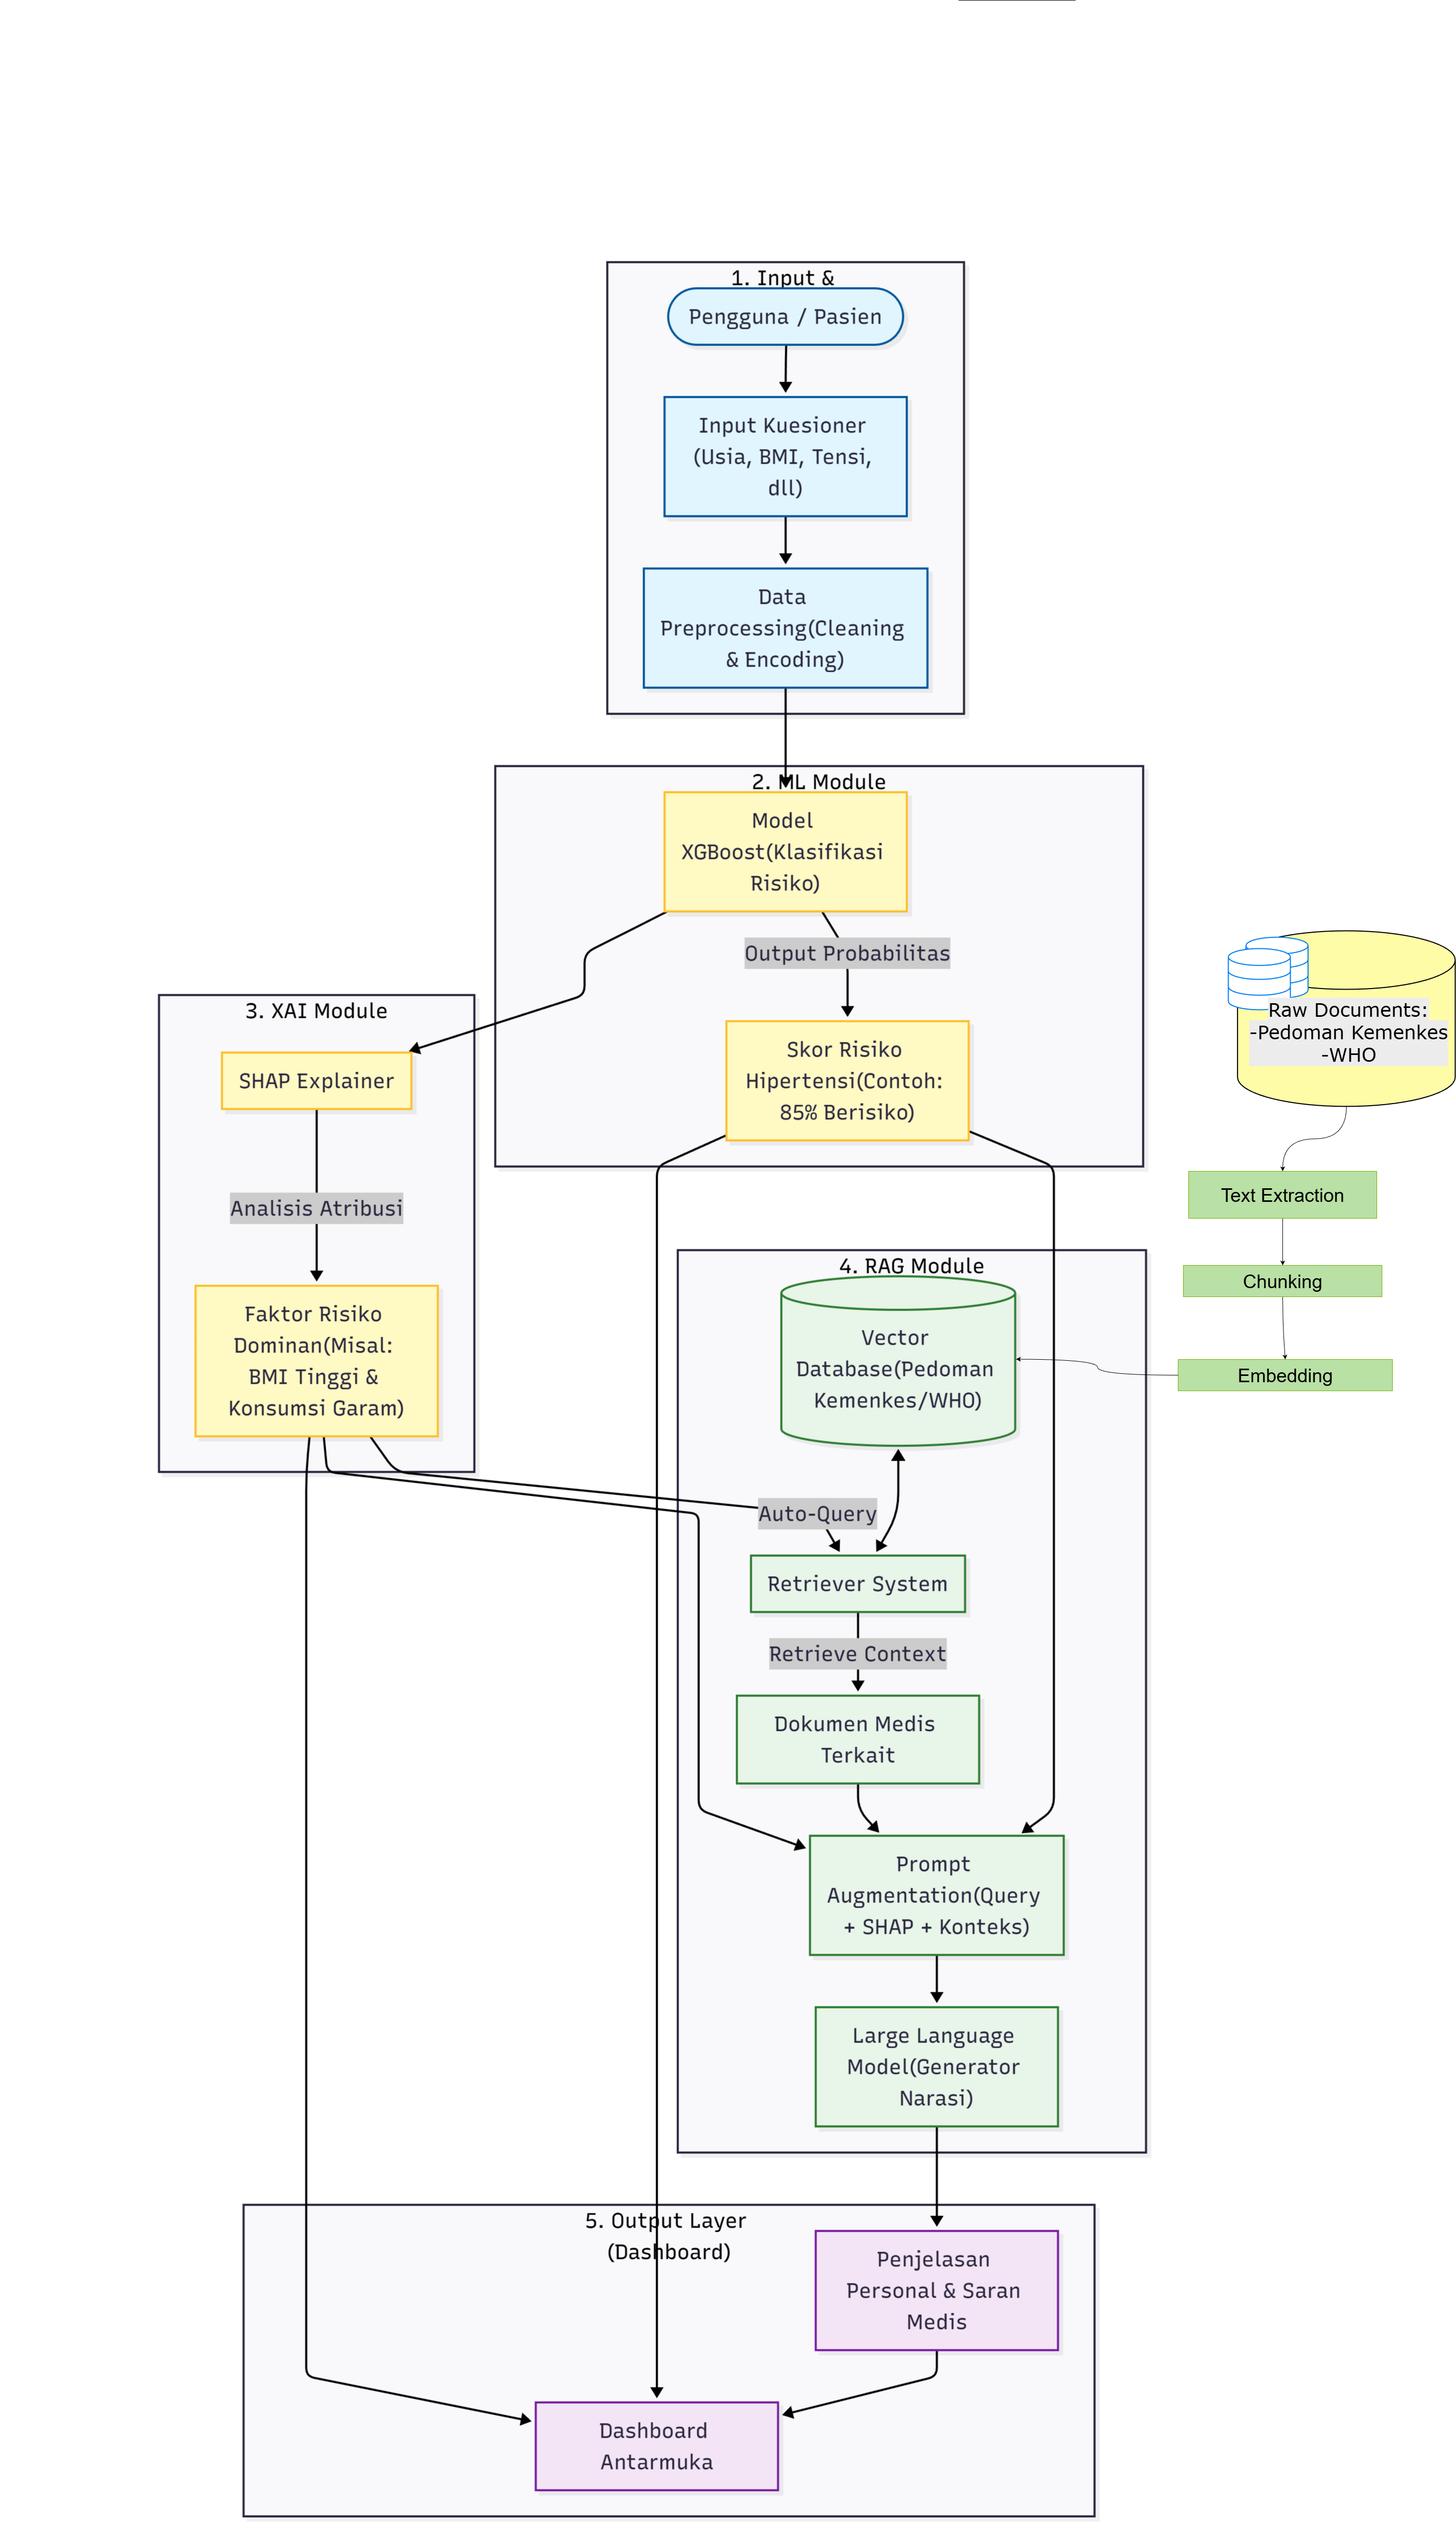
\includegraphics[width=0.8\textwidth]{images/Desain Konsep Solusi.png} 
    \caption{Desain Konsep Solusi Sistem}
    \label{fig:konsep-solusi}
\end{figure}
Berikut ini adalah uraian komponen pada desain sistem:


\begin{enumerate}
    \item \textit{Input Layer \& Preprocessing} \\
    Komponen ini berfungsi sebagai antarmuka akuisisi data yang menerima variabel input mentah dari pengguna. Sebelum masuk ke model, data tabular melalui pipa pra-pemrosesan (\textit{preprocessing pipeline}) yang ketat menggunakan pustaka manipulasi data (seperti \textit{Pandas}). Proses ini mencakup dua mekanisme utama:
    \begin{itemize}
        \item \textit{Value Imputation}: Sistem mendeteksi \textit{null values} dan melakukan imputasi (misalnya menggunakan \textit{mean/median} atau menghapus baris) untuk menjaga integritas matriks fitur.
        \item \textit{Feature Encoding}: Model matematis seperti ML hanya dapat memproses angka, sehingga variabel kategorikal harus dikonversi menjadi format numerik. Untuk variabel biner dan ordinal seperti jenis kelamin atau tingkat aktivitas, diterapkan teknik \textit{label encoding} yang memetakan kategori ke integer.
    \end{itemize}

    \item \textit{ML Module} \\
    Modul ini bertindak sebagai mesin inferensi yang menjalankan algoritma \textit{Machine Learning}. Secara teknis, model ini bekerja dengan membangun \textit{ensemble} dari pohon keputusan (\textit{decision trees}) secara sekuensial, di mana setiap pohon baru memperbaiki residu kesalahan (\textit{error residual}) dari pohon sebelumnya.
    \begin{itemize}
        \item \textit{Kalkulasi Probabilitas}: Model menghasilkan luaran berupa nilai \textit{log-odds} (\textit{logit}) yang kemudian ditransformasi menggunakan fungsi \textit{sigmoid} untuk menghasilkan skor probabilitas kontinu antara 0 hingga 1.
        \item \textit{Penentuan Kelas}: Probabilitas tersebut dikomparasi terhadap ambang batas (\textit{threshold}) keputusan (biasanya 0.5 atau disesuaikan demi sensitivitas) untuk mengklasifikasikan label akhir menjadi "Berisiko" atau "Tidak Beresiko".
    \end{itemize}

    \item \textit{XAI Module} \\
    Modul ini menerapkan metode XAI untuk mengaudit keputusan model. Secara matematis, modul ini menghitung nilai \textit{Shapley}, yaitu kontribusi marginal rata-rata dari setiap fitur terhadap selisih antara prediksi aktual instans tersebut dengan prediksi rata-rata dasar.
    \begin{itemize}
        \item \textit{Output Atribusi}: Hasilnya adalah vektor nilai XAI untuk setiap fitur (positif atau negatif), yang menunjukkan seberapa besar dan ke arah mana (menaikkan atau menurunkan risiko) fitur tersebut mempengaruhi skor probabilitas pasien secara spesifik.
    \end{itemize}

    \item \textit{RAG Module} \\
    Modul ini terdiri dari dua fase utama, yaitu \textit{Ingestion} dan \textit{Retrieval \& Generation}.
    \begin{enumerate}[label=\Alph*.]
        \item \textit{Ingestion} \\
        Proses ini mengubah dokumen statis menjadi struktur data yang dapat dicari secara semantik oleh mesin:
        \begin{itemize}
            \item \textit{Raw Documents}: Sistem mengumpulkan dokumen pedoman klinis resmi, seperti panduan hipertensi dari Kemenkes RI atau WHO, dalam format PDF atau teks digital. Dokumen ini menjadi \textit{ground truth} atau sumber kebenaran tunggal.
            \item \textit{Text Extraction}: Karena mesin tidak bisa membaca visual PDF secara langsung, proses ekstraksi dilakukan menggunakan teknik OCR atau \textit{parsing} untuk memisahkan konten teks murni dari elemen \textit{layout}, gambar, atau \textit{header/footer} yang tidak relevan.
            \item \textit{Chunking}: Teks hasil ekstraksi tidak langsung diproses utuh karena keterbatasan \textit{context window} pada model bahasa. Teks dipecah menjadi segmen-segmen kecil atau \textit{chunks}, misalnya per paragraf atau per 512 token untuk mempertahankan granularitas konteks. Semakin spesifik potongan dari \textit{chunks}, semakin akurat nanti pencariannya.
            \item \textit{Embedding}: Setiap \textit{chunk} teks dikonversi menjadi representasi numerik berupa vektor berdimensi tinggi, misalnya \textit{array} berisi 1536 angka \textit{float}, menggunakan model \textit{embedding}. Vektor ini merepresentasikan makna semantik dari teks tersebut. Kalimat dengan makna serupa akan memiliki nilai vektor yang berdekatan secara matematis.
            \item \textit{Vector Database}: Vektor-vektor tersebut kemudian diindeks dan disimpan dalam \textit{Vector Database} yang dioptimalkan untuk operasi pencarian jarak yang berkecepatan tinggi, bukan pencarian kata kunci biasa.
        \end{itemize}

        \item \textit{Retrieval \& Generation} \\
        Fase ini terjadi secara \textit{real-time} saat pengguna meminta prediksi:
        \begin{itemize}
            \item \textit{Auto-Query}: Ini adalah komponen yang menjembatani hasil analisis XAI dengan pencarian referensi. Sistem secara otomatis menyusun kueri pencarian berdasarkan luaran modul XAI, bukan sekadar meneruskan input mentah pengguna. Sebagai contoh, jika pengguna hanya memasukkan data "umur 50", \textit{Auto-Query} akan mengambil konteks "Usia Lanjut" dan "Hipertensi" dari analisis risiko untuk membentuk kueri spesifik: "Bagaimana pengaruh usia lanjut terhadap risiko hipertensi menurut pedoman medis?"
            \item \textit{Retriever System}: Sistem penerima kueri ini melakukan pencarian kesamaan (\textit{similarity search}) ke dalam \textit{Vector Database}. Sistem membandingkan vektor dari \textit{Auto-Query} dengan jutaan vektor dokumen yang tersimpan menggunakan perhitungan \textit{Cosine Similarity} atau \textit{Euclidean Distance}.
            \item \textit{Retrieve Context}: Hasil dari \textit{Retriever} bukanlah jawaban, melainkan potongan dokumen (\textit{chunks}) yang memiliki skor kemiripan tertinggi dengan kueri. Konteks ini diambil untuk memberikan "bahan bacaan" yang valid bagi LLM.
            \item \textit{Prompt Augmentation}: Di sini sistem menggabungkan tiga elemen menjadi satu instruksi lengkap: (1) Kueri Asli, (2) Hasil Analisis SHAP (Faktor Risiko), dan (3) \textit{Retrieved Context} (Dokumen Pedoman). Teknik ini disebut \textit{In-Context Learning}, di mana kita memaksa model untuk menjawab hanya berdasarkan konteks yang kita suapkan.
            \item \textit{Large Language Model (Generator)}: Terakhir, LLM memproses \textit{prompt} yang sudah diperkaya (\textit{augmented}) tersebut untuk menyusun narasi bahasa alami yang koheren, personal, dan tervalidasi oleh dokumen medis yang dilampirkan dalam konteks.
        \end{itemize}
    \end{enumerate}
\end{enumerate}
\subsection{Alur Kerja Sistem}
Gambar \ref{fig:alur-kerja} mengilustrasikan alur kerja dari sistem yang dirancang.

\begin{figure}[H]
    \centering
    % Pastikan nama file tidak menggunakan spasi. Gunakan underscore atau dash.
    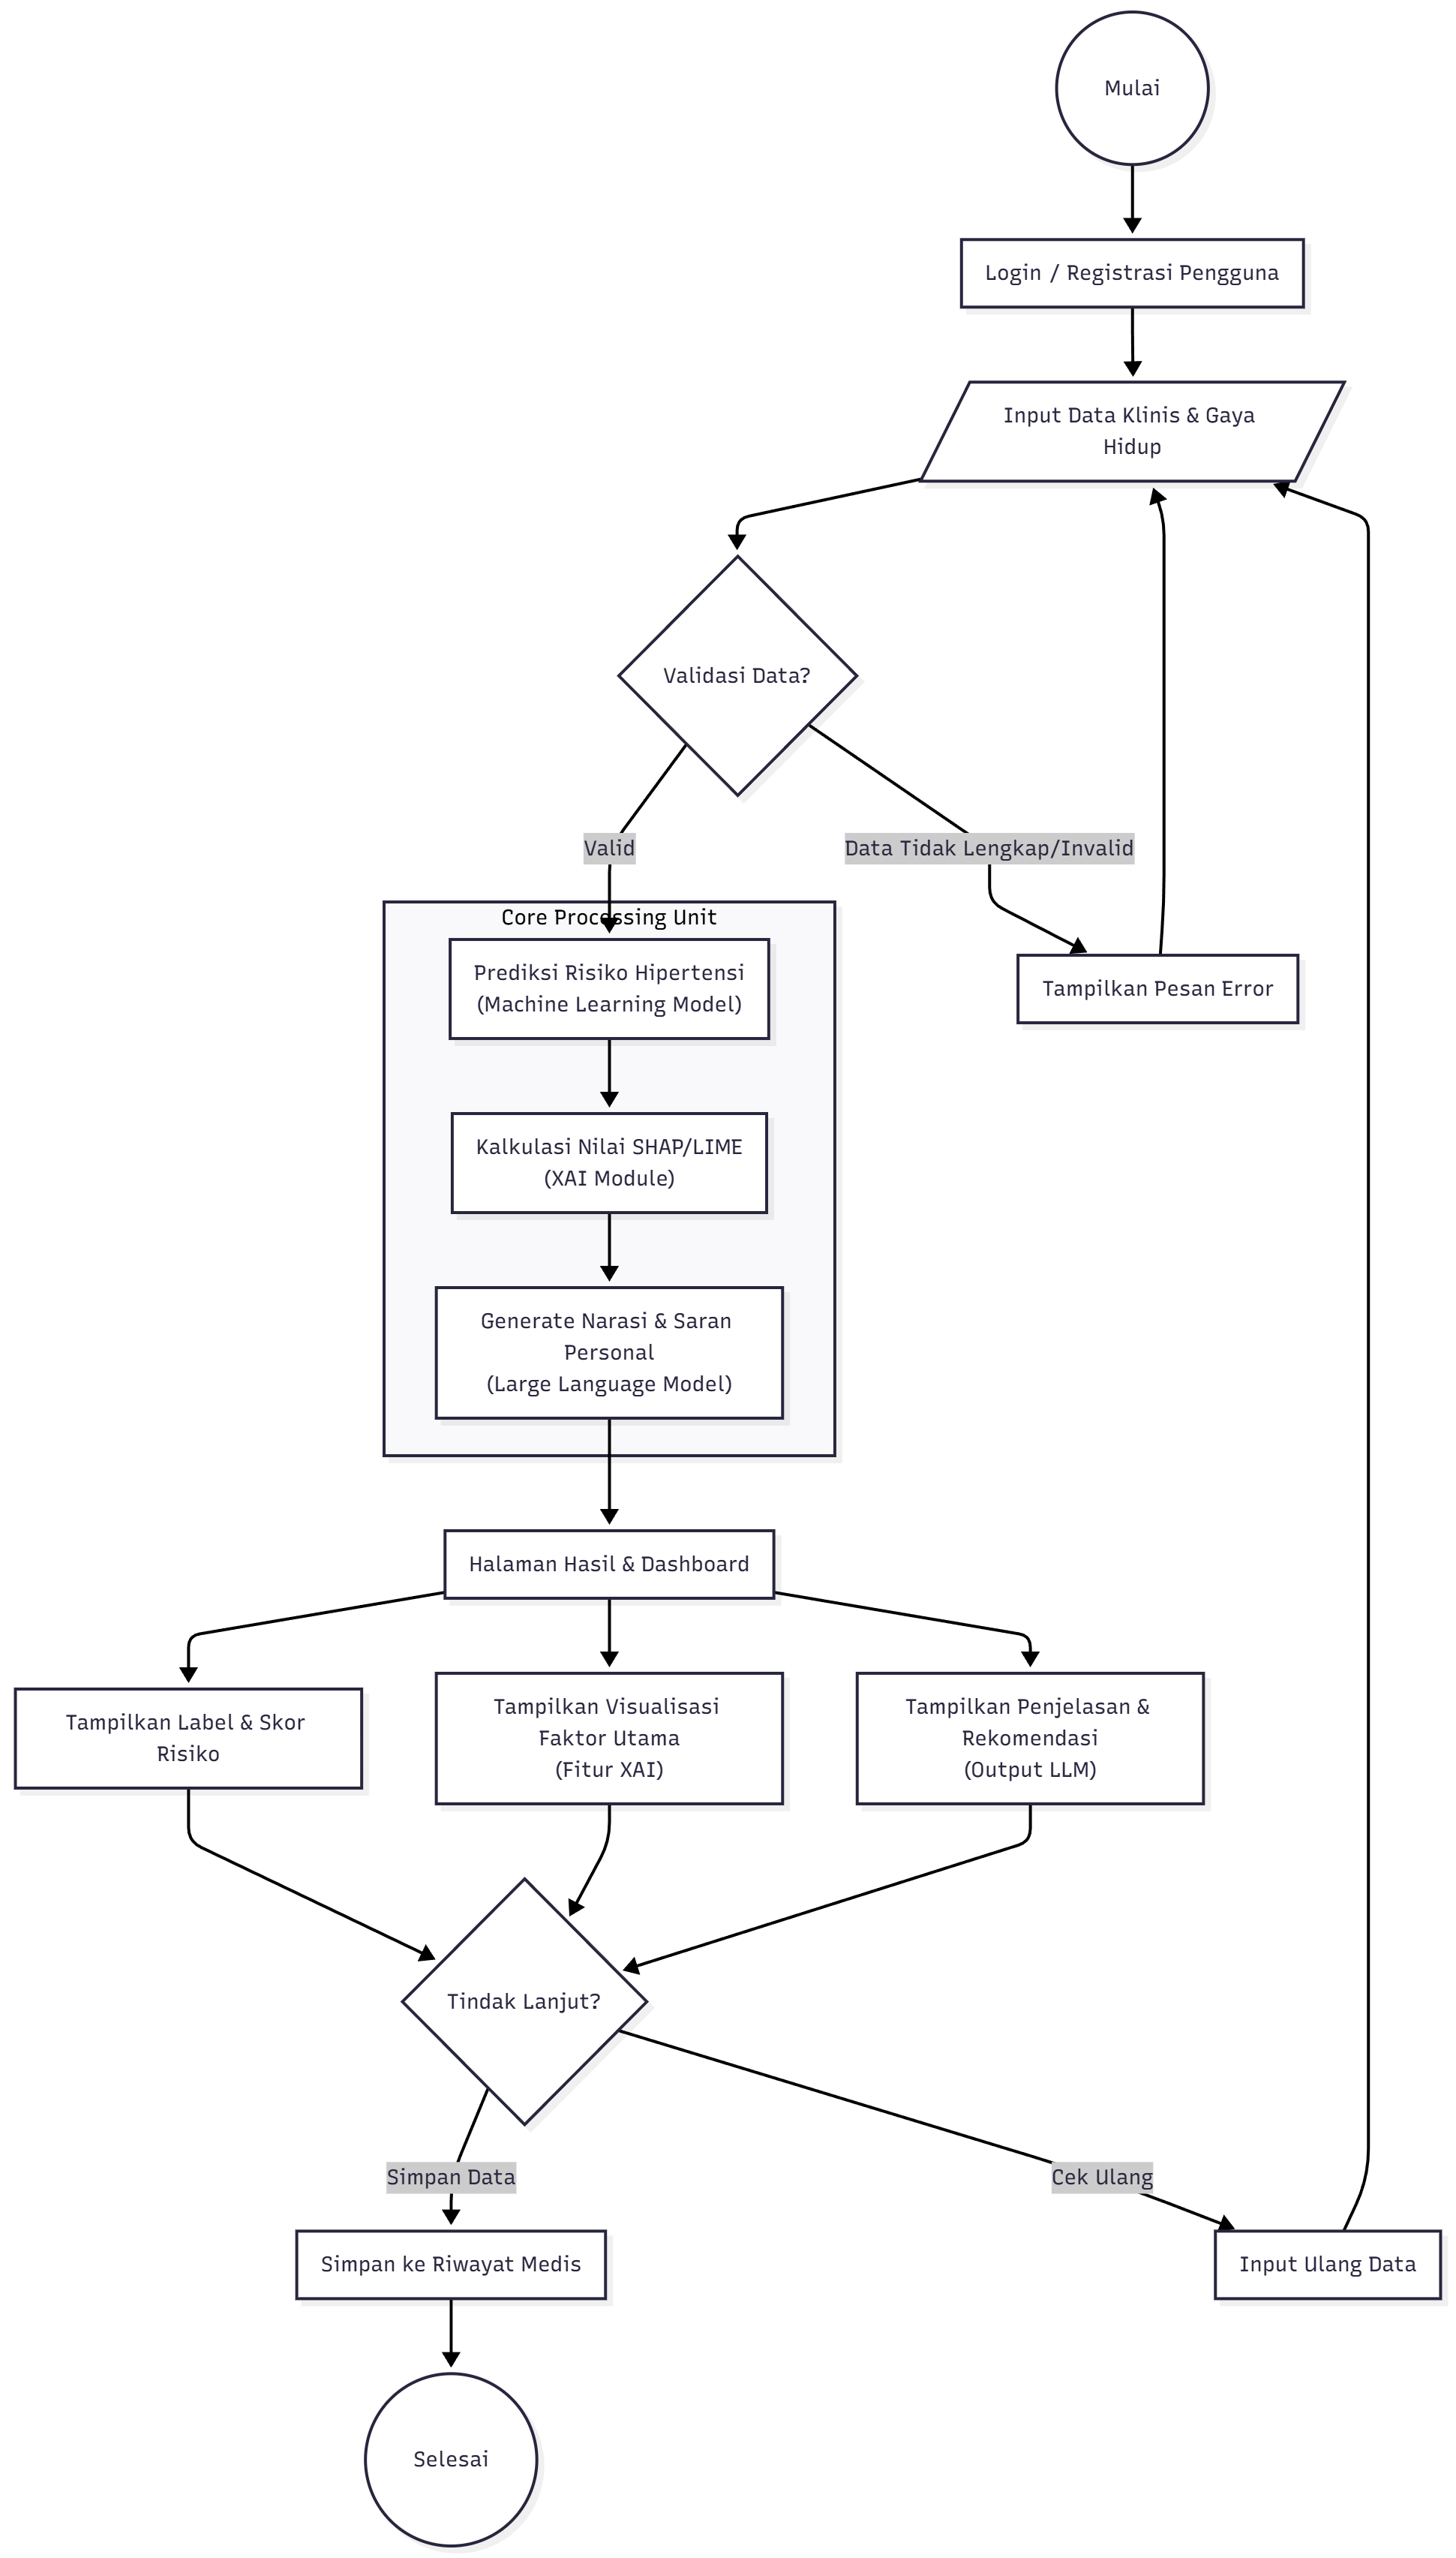
\includegraphics[width=0.8\textwidth]{images/alur kerja sistem.png} 
    \caption{Gambar Alur Kerja Sistem}
    \label{fig:alur-kerja}
\end{figure}
Sistem yang diusulkan bekerja dalam alur sebagai berikut:

\begin{enumerate}
    \item Pengguna memasukkan parameter kesehatan seperti usia, tekanan darah, IMT, dan riwayat keluarga pada kuesioner di sistem.
    
    \item Model ML memproses data tersebut untuk menghasilkan skor probabilitas risiko hipertensi (misalnya: 56\% Berisiko).
    
    \item Secara paralel, modul XAI menghitung nilai atribusi fitur yang mendasar keputusan \textit{black box} model ML. Modul ini mengidentifikasi variabel mana yang paling berkontribusi terhadap skor risiko tersebut, misalnya tinggi konsumsi garam dan IMT, yang menjadi kontributor utama.
    
    \item Sistem mengambil hasil atribusi fitur dari SHAP. Lalu setelahnya, sistem melakukan pencarian (\textit{retrieval}) pada basis data vektor yang berisi pedoman medis yang relevan dengan faktor risiko yang ditemukan, seperti pedoman dari Kemenkes atau WHO. LLM akan menggabungkan hasil prediksi, alasan dari SHAP, dan referensi medis untuk menyusun narasi penjelasan yang personal dan valid.
    
    \item Pengguna menerima tiga luaran terintegrasi: Status Risiko (ML), Grafik Faktor Penyebab (XAI), dan Penjelasan Naratif serta Saran Medis (RAG-LLM).
\end{enumerate}

\subsection{Arsitektur Sistem}
Diagram arsitektur sistem diperlukan untuk memetakan bagaimana komponen perangkat lunak, aliran data, dan infrastruktur saling berinteraksi guna menjalankan logika prediksi secara stabil, aman, dan skalabel.

Gambar \ref{fig:arsitektur-teknis} berikut mengilustrasikan arsitektur teknis sistem yang dirancang dengan pendekatan berbasis layanan (\textit{service-based architecture}).

\begin{figure}[H]
    \centering
    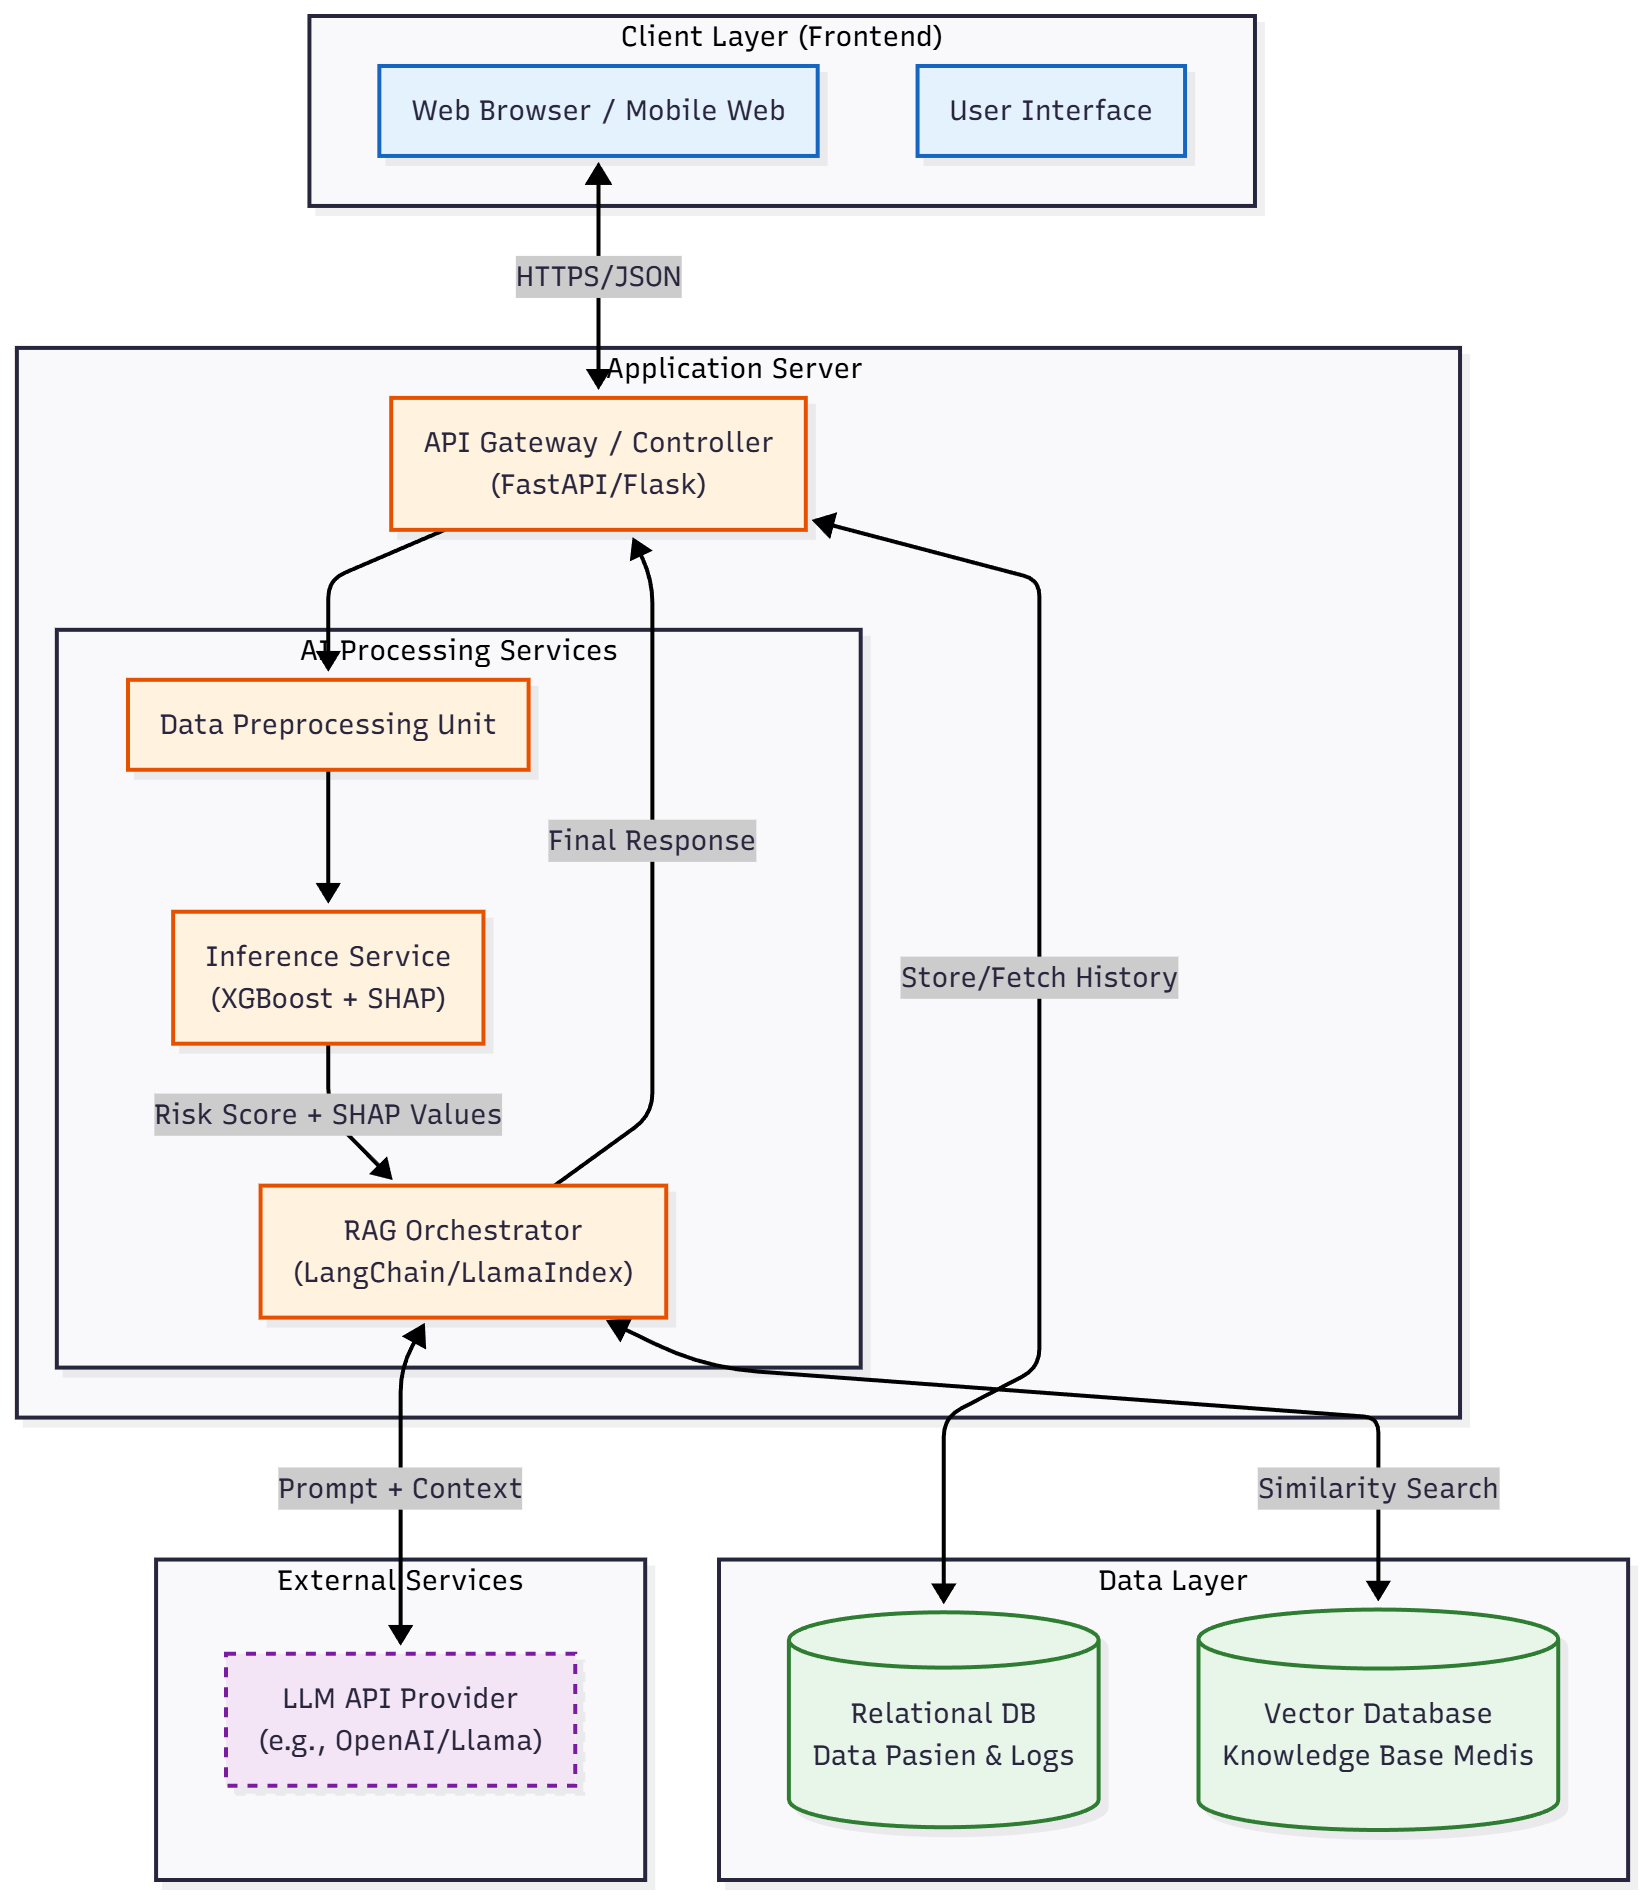
\includegraphics[width=0.8\textwidth]{images/arsitektur sistem.png}
    \caption{Arsitektur Teknis Sistem }
    \label{fig:arsitektur-teknis}
\end{figure}

Berdasarkan Gambar \ref{fig:arsitektur-teknis} di atas, sistem terbagi menjadi empat lapisan utama dengan fungsi spesifik sebagai berikut:

\begin{itemize}
    \item Client Layer (Frontend) \\
    Lapisan ini merupakan titik interaksi pengguna, baik melalui peramban web desktop maupun perangkat seluler. Lapisan ini bertugas menangkap input data klinis pasien dan memvisualisasikan hasil prediksi berupa grafik risiko dan narasi penjelasan yang dikirimkan oleh server melalui protokol HTTPS/JSON yang aman.

    \item Application Layer \\
    Lapisan ini berfungsi sebagai otak pemrosesan sistem. Lapisan ini terdiri dari API Gateway yang mengatur lalu lintas data, serta unit AI Processing Services yang menjalankan tiga fungsi sekuensial:
    \begin{enumerate}
        \item \textit{Data Preprocessing} untuk membersihkan input.
        \item \textit{Inference Service} yang menjalankan model XGBoost dan SHAP untuk menghitung skor risiko.
        \item \textit{RAG Orchestrator} yang meramu \textit{prompt} untuk model bahasa.
    \end{enumerate}

    \item Data Layer \\
    Lapisan ini bertanggung jawab atas persistensi data dengan menggunakan dua jenis basis data. \textit{Relational Database} digunakan untuk menyimpan data terstruktur pasien dan log riwayat prediksi, sedangkan \textit{vector database} digunakan khusus untuk menyimpan \textit{embedding} dokumen pedoman medis yang memungkinkan pencarian konteks semantik (\textit{similarity search}) yang cepat.

    \item External Services \\
    Sistem terhubung dengan penyedia layanan \textit{Large Language Model} (LLM) pihak ketiga seperti OpenAI atau model \textit{open-source} terhosting lainnya. Komponen ini menerima \textit{prompt} yang telah diperkaya dengan konteks medis dari sistem internal untuk menghasilkan narasi penjelasan yang natural, namun tetap tervalidasi.
\end{itemize}

\section{Perbandingan dengan Sistem Saat Ini}
Desain konsep solusi di atas menawarkan perubahan paradigma dari pendekatan konvensional yang digambarkan pada Bab III menjadi pendekatan berbasis kecerdasan buatan yang terintegrasi. Perbandingan komparatif antara kondisi saat ini (\textit{As-Is}) dan solusi yang diusulkan (\textit{To-Be}) dirangkum dalam Gambar \ref{fig:alur-diagnosis}.

% \begin{table}[htbp]
%     \centering
%     \caption{Perbandingan Sistem Konvensional vs Sistem Usulan}
%     \label{tab:perbandingan-sistem}
%     \renewcommand{\arraystretch}{1.5} % Menambah jarak antar baris agar lebih rapi
%     \begin{tabular}{|p{3.5cm}|p{5.5cm}|p{5.5cm}|}
%     \hline
%     \textbf{Aspek Pembanding} & \textbf{Sistem Saat Ini (As-Is)} & \textbf{Solusi Usulan (To-Be)} \\
%     \hline
%     Pendekatan Diagnosis & 
%     Reaktif \& Manual. Diagnosis bergantung pada pengukuran sesaat di klinik dan ingatan dokter terhadap pedoman. & 
%     Prediktif \& Otomatis. Sistem memprediksi risiko secara dini berdasarkan pola data historis menggunakan \textit{Machine Learning}. \\
%     \hline
%     Transparansi Keputusan & 
%     Intuitif/Implisit. Keputusan dokter didasarkan pada \textit{tacit knowledge} yang sulit dijelaskan secara kuantitatif kepada pasien. & 
%     \textit{Explainable} (XAI). Sistem menyediakan visualisasi atribusi fitur (SHAP) yang menunjukkan secara persis variabel penyebab risiko secara matematis. \\
%     \hline
%     Penyampaian Informasi & 
%     Lisan \& Terbatas. Penjelasan risiko sering kali singkat karena keterbatasan waktu konsultasi, menyebabkan pasien kurang paham. & 
%     Narasi Personal (GenAI). LLM menghasilkan penjelasan tertulis yang disesuaikan dengan profil pasien, menjabarkan hubungan sebab-akibat dengan bahasa alami. \\
%     \hline
%     Validitas Referensi & 
%     Variatif. Sangat bergantung pada \textit{update} pengetahuan tenaga medis masing-masing. & 
%     Terstandarisasi (RAG). Setiap saran yang dihasilkan divalidasi silang (\textit{cross-reference}) dengan dokumen pedoman medis terkini di \textit{Vector Database}. \\
%     \hline
%     Alur Kerja & 
%     Linear dan membutuhkan eskalasi manual bertingkat (perawat $\rightarrow$ dokter). & 
%     Terintegrasi dan \textit{real-time}, memberikan \textit{second opinion} instan sebelum eskalasi ke ahli. \\
%     \hline
%     \end{tabular}
% \end{table}

\begin{figure}[H]
    \centering
    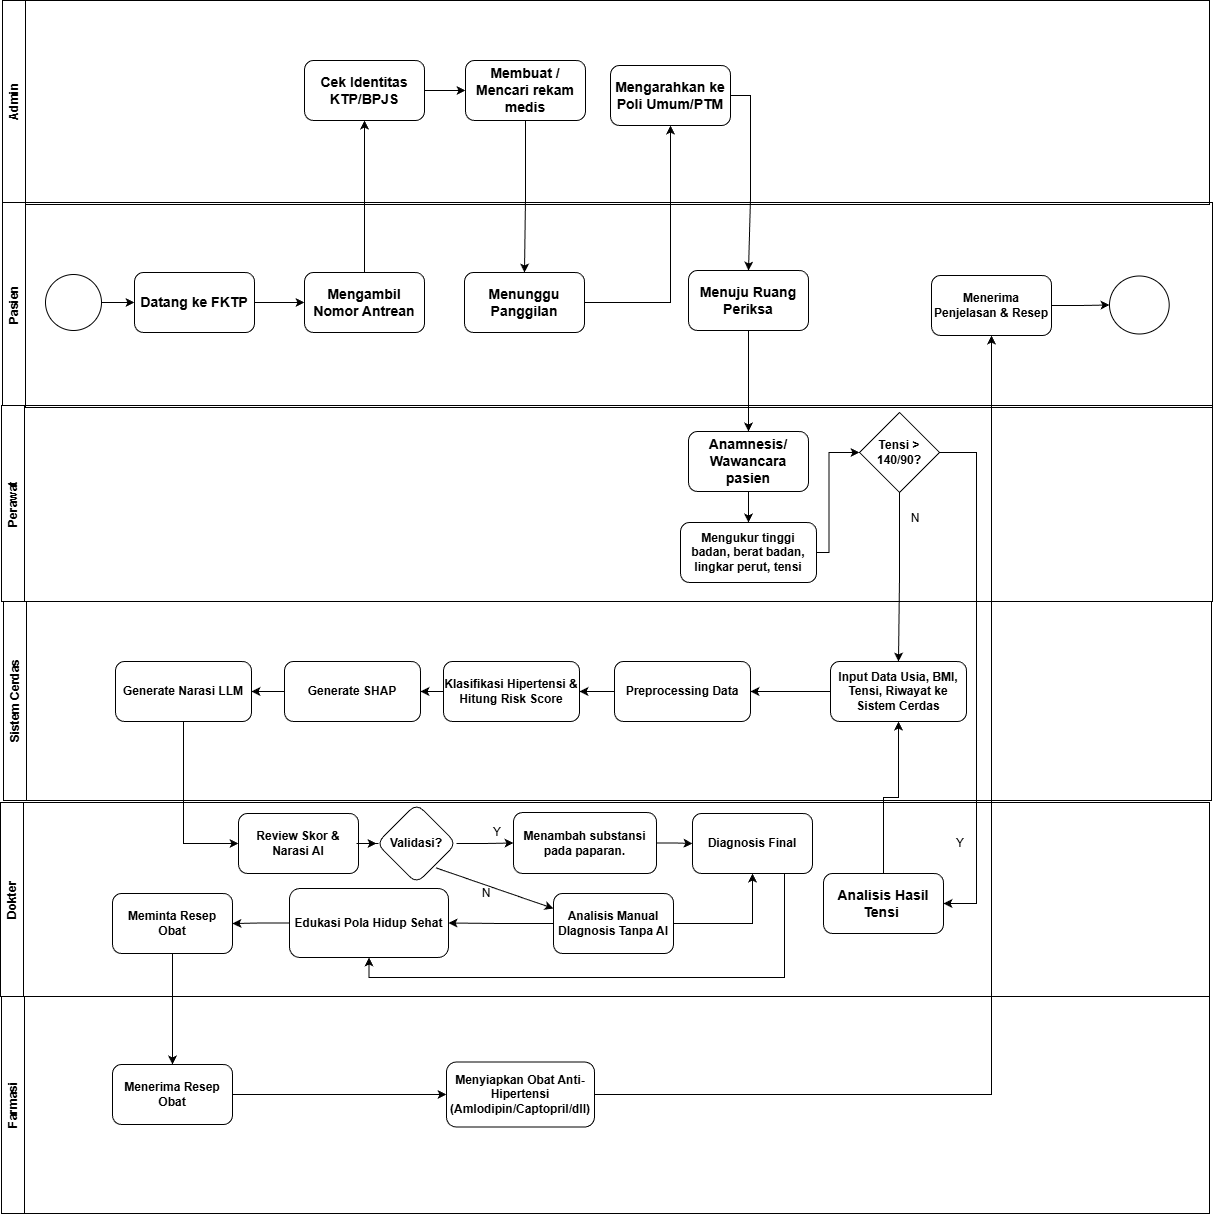
\includegraphics[width=0.8\textwidth]{images/alursistemtobe.png}
    \caption{Alur Diagnosis Hipertensi di Fasilitas Kesehatan Tingkat Pertama (FKTP) (To-Be)}
    \label{fig:alur-diagnosis}
\end{figure}

Secara visual, jika dibandingkan dengan kondisi awal, desain usulan menggambarkan adanya otomatisasi dalam proses penalaran klinis. Pada tahap ini, dokter tidak lagi melakukan observasi data pasien secara manual, melainkan memasukkan data tersebut ke dalam sistem yang berfungsi sebagai pendukung dalam pengambilan keputusan.

Meskipun demikian, penekanan utama tetap berada pada peran dokter sebagai pengambil keputusan akhir. Informasi maupun rekomendasi yang diberikan sistem harus dipahami, ditafsirkan, dan dievaluasi kembali oleh dokter untuk memperoleh wawasan klinis yang komprehensif. Dengan demikian, sistem ini dirancang bukan untuk menggantikan fungsi dokter dalam menentukan keputusan medis, tetapi untuk mengurangi beban kognitif dalam proses analisis data sehingga dokter dapat membuat keputusan yang lebih tepat, efisien, dan berbasis informasi.